\definecolor{darkblue}{rgb}{0.0,0.0,0.5}
\definecolor{darkgreen}{rgb}{0.0,0.5,0.0}
% Macro for code snippets
\newcommand{\ccode}[4]
{
  \begin{block}{#3}
%  \vspace{-5mm}
  \lstinputlisting[basicstyle=\sffamily\footnotesize,language=C,
                   keywordstyle={\color{darkgreen}\bf},
                   commentstyle=\color{darkblue},
                   showspaces=false, showstringspaces=false,
                   firstline={#1},lastline={#2}]{#4}
  \end{block}
}
%
% Document
%
\title[]{High-performance processing and development with Madagascar}

%\author[Bashkardin]{Vladimir Bashkardin}
\institute[RSF-dev team]{Madagascar development team}
\date[Madagascar school in Houston] % (optional)
{July 24, 2010}

\setbeamercolor{alerted text}{fg=white}
\begin{frame}
  \titlepage
  % Hide progress bar in the footline
  \appendix
\end{frame}

\begin{frame}
  \frametitle{Outline}
   \hspace*{2cm}
   \begin{minipage}[t][4.5cm]{10cm}
    \tableofcontents
   \end{minipage}
\end{frame}

\section{HPC terminology and frameworks}

\begin{frame}
%  \vspace{1.0cm}
  \begin{figure}
  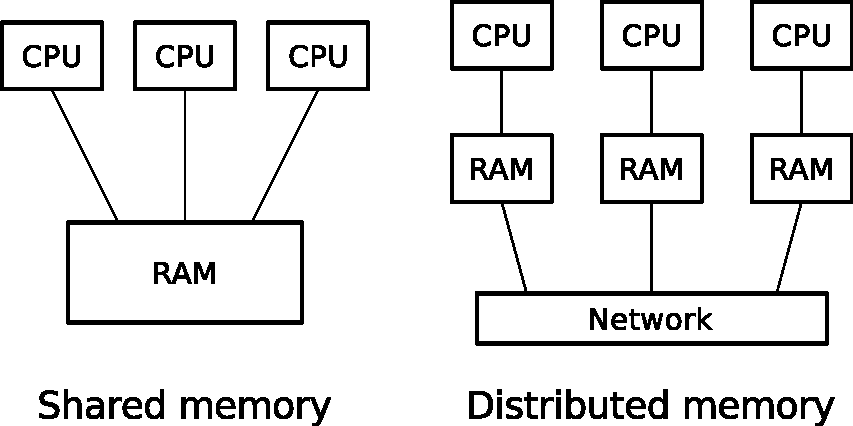
\includegraphics[scale=0.65]{Fig/hpc.pdf}
  \end{figure}
  \begin{block}{}
    \begin{itemize}
      \item Vast majority of modern HPC systems are hybrid
      \item Rise of GPUs added another level of hardware and software complexity
    \end{itemize}
  \end{block}
\end{frame}

\begin{frame}
  \begin{block}{Application frameworks for HPC}
  \begin{table}
    \begin{center}
     \begin{tabular}{|c|c|c|}
      \hline               &       Type       &   Supported via       \\
      \hline & & \\[-1em]
      \hline     OpenMP    &      Shared      & Compiler pragmas      \\
      \hline       MPI     &   Distributed    &    Libraries\footnote[1]
      {Executables need special environment to run: remote shell + launcher (mpirun)} \\
      \hline     GPU/CUDA  & Special hardware & Extra compiler + SDK\footnote[2]
      {Executables need proprietary drivers to run GPU kernels, but can be recompiled in emulation mode}  \\
      \hline
    \end{tabular}
   \end{center}
  \end{table}
  \end{block}
  \begin{block}{}
    \begin{itemize}
      \item Most big clusters have job batch systems. On such systems, programs cannot be run directly,
but have to be submitted to a queue.
    \end{itemize}
  \end{block}
\end{frame}

\begin{frame}
  \begin{block}{Design goals for HPC support}
    \begin{itemize}
      \item Support for all combination of systems
      \item Fault tolerance and portability of SConstructs
    \end{itemize}
  \end{block}
  \begin{block}{How?}
    \begin{itemize}
      \item Utilize explicit (data) parallelism whenever possible: keep basic
            programs simple and sequential, handle parallelization inside
            {\bf Flow}() statements automatically
      \item Define system-dependent execution parameters outside of SConstructs
    \end{itemize}
  \end{block}
\end{frame}

\section{Utilizing data parallelism}

\begin{frame}
  \begin{block}{How to define parallel {\bf Flow}()}
    {\bf Flow}('target','source','workflow',[n,m],reduce='cat') \\
    \# Process 'source' independently along {\bf n}th dimension of length {\bf m},
    concatenate all results into 'target'.
  \end{block}
  \begin{block}{How to run}
    \$ export {\bf RSF\_THREADS}='{\bf 16}' \\
    \$ export {\bf RSF\_CLUSTER}='hostname1 {\bf 8} hostname2 {\bf 8}' \\
    \$ pscons \# or \\
    \$ scons -j {\bf 16} {\bf CLUSTER}='hostname1 {\bf 8} hostname2 {\bf 8}'
  \end{block}
  \begin{block}{What happens inside}
%    \vspace{-5mm}
    \begin{enumerate}
      \item Source file gets split into several independent temporary files
      \item SCons executes same workflow on cluster nodes for each file
            independently through remote shell (ssh)
      \item SCons assembles independent outputs into one target
    \end{enumerate}
  \end{block}
\end{frame}

\begin{frame}
%  \vspace{1.25cm}
  \begin{figure}
  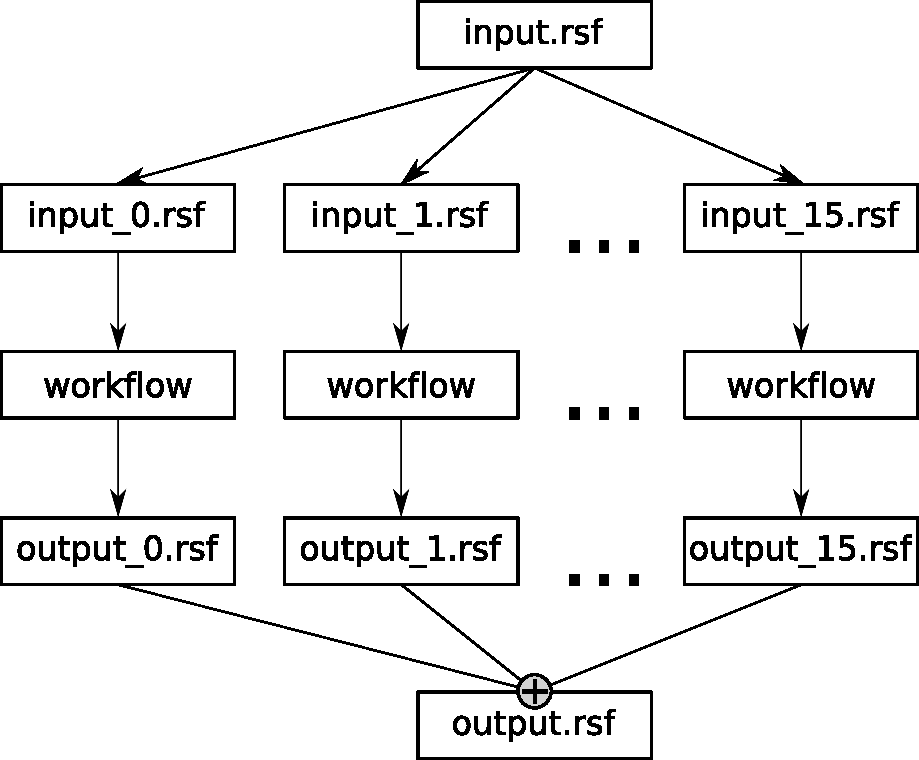
\includegraphics[scale=0.45]{Fig/pscons.pdf}
  \caption{Parallel workflows with PSCons}
  \end{figure}
\end{frame}

\begin{frame}
  \begin{block}{Scratch directory for tmp files}
    \$ export {\bf TMPDATAPATH}=/local/fast/file/system
  \end{block}
  \begin{block}{Monitor running programs}
    \$ sftop
  \end{block}
  \begin{block}{Kill remote programs}
    \$ sfkill sfprogram
  \end{block}
\end{frame}

\begin{frame}
  \begin{block}{Fallbacks}
    If remote shell is not available directly, then it is possible to try to
    bypass it.
  \end{block}
  \begin{block}{Directly through MPI}
    {\bf Flow}('target','source','workflow',[n,'mpi'],np=m,reduce='cat') \\
    \# Try to invoke MPI executable environment directly with {\bf mpirun} -np
    {\bf m}.
  \end{block}
  \begin{block}{Directly through OpenMP}
    {\bf Flow}('target','source','workflow',[n,'omp'],reduce='cat') \\
    \# Try to run the workflow in OpenMP environment locally.
  \end{block}
  \begin{block}{Note}
    These options are not as portable as the general one.
  \end{block}
\end{frame}

\section{HPC development with Madagascar}

\begin{frame}
  \begin{block}{'Hello World' program of HPC world}
    \[ \mathbf{c} = \mathbf{a} + \mathbf{b}. \]
%    \vspace{2mm}
  \end{block}
  \begin{figure}
  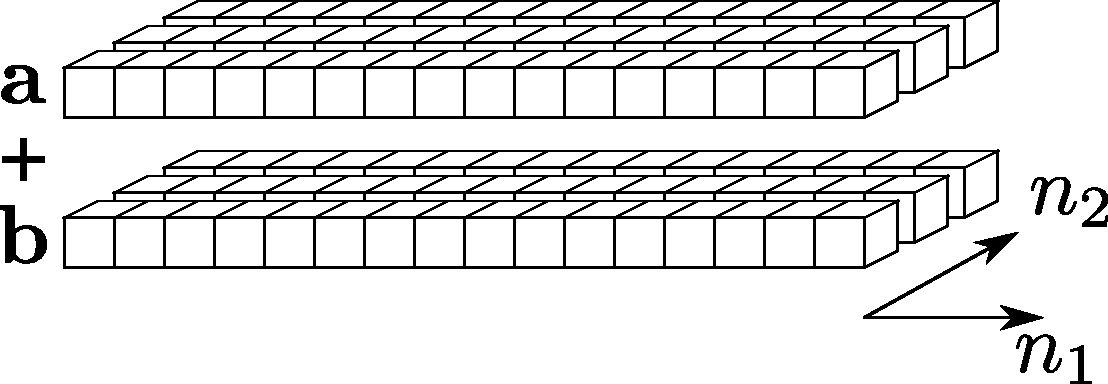
\includegraphics[scale=0.35]{Fig/abcfig.pdf}
  \end{figure}
  \begin{block}{Approaches}
    \begin{itemize}
%      \vspace{-2mm}
      \item First, the obvious one - {\bf pscons}
      \item Then, let us assume that this problem is not data parallel and
explicit parallellism has to be expressed at the level of source code
    \end{itemize}
  \end{block}
\end{frame}

\begin{frame}
  \begin{block}{Obvious solution}
%  \vspace{-5mm}
  \lstinputlisting[basicstyle=\sffamily\footnotesize,language=Python,
                   keywordstyle={\color{darkgreen}\bf},
                   commentstyle=\color{darkblue},
                   showspaces=false, showstringspaces=false]{pscons/SConstruct}
  \end{block}
  \begin{block}{How to run}
    \$ pscons
  \end{block}
  \begin{block}{Note}
%    \vspace{-5mm}
    \begin{itemize}
      \item This approach will work on any type of system and on a
single-CPU machine as well
      \item Splitting inputs and collecting outputs add overhead
    \end{itemize}
  \end{block}
\end{frame}

\begin{frame}
  \begin{block}{vecsum.job - job file for running inside LSF batch system}
  \lstinputlisting[basicstyle=\sffamily\footnotesize,language=bash,
                   keywordstyle={\color{darkgreen}\bf},
                   commentstyle=\color{darkblue},
                   showspaces=false, showstringspaces=false]{pscons/vecsum.job}
  \end{block}
  \begin{block}{How to run}
    \$ bsub \textless vecsum.job
  \end{block}
\end{frame}

\subsection{OpenMP}

\begin{frame}
%  \vspace{1.0cm}
  \begin{figure}
  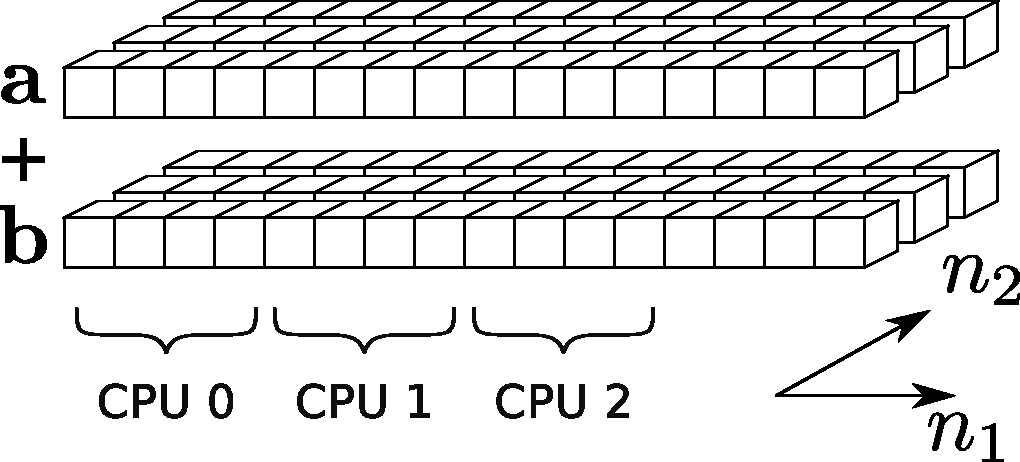
\includegraphics[scale=0.55]{Fig/abcomp.pdf}
  \caption{Summation of vectors with OpenMP}
  \end{figure}
\end{frame}

\begin{frame}
  \ccode{20}{37}{omphello.c}{omp/omphello.c}
\end{frame}
\begin{frame}
  \ccode{38}{59}{omphello.c}{omp/omphello.c}
\end{frame}

\begin{frame}
  \begin{block}{How to compile}
    Like any regular Madagascar program. 
  \end{block}
  \begin{block}{How to run}
    \$ scons/pscons
  \end{block}
  \begin{block}{Note}
    \begin{itemize}
      \item Even if OpenMP is not supported, the source code will get
compiled as sequential
      \item It can be combined with upper-level parallelization in SConstruct
      \item For a good real-life example, look into RSFSRC/user/psava/sfawefd.c
    \end{itemize}
  \end{block}
\end{frame}

\subsection{MPI}

\begin{frame}
%  \vspace{1.0cm}
  \begin{figure}
  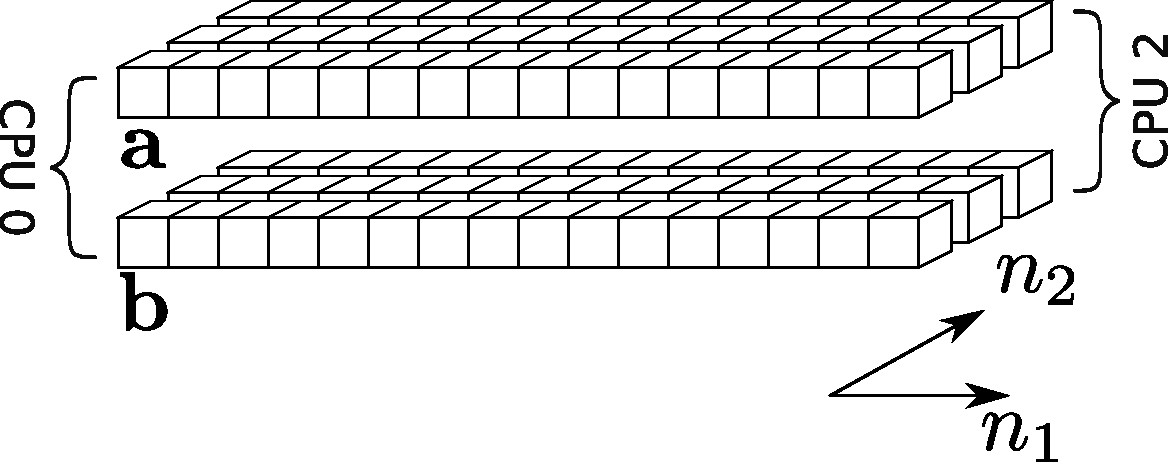
\includegraphics[scale=0.55]{Fig/abcmpi.pdf}
  \caption{Summation of vectors with MPI}
  \end{figure}
\end{frame}

\newcommand{\RSFSRC}{../../..}

\begin{frame}
  \ccode{20}{37}{mpihello.c}{\RSFSRC/user/bash/Mmpihello.c}
\end{frame}
\begin{frame}
  \ccode{38}{56}{mpihello.c}{\RSFSRC/user/bash/Mmpihello.c}
\end{frame}
\begin{frame}
  \ccode{58}{77}{mpihello.c}{\RSFSRC/user/bash/Mmpihello.c}
\end{frame}
\begin{frame}
  \ccode{78}{96}{mpihello.c}{\RSFSRC/user/bash/Mmpihello.c}
\end{frame}

\begin{frame}
  \begin{block}{How to compile}
    Look into RSFSRC/system/main/SConstruct for mpi.c 
  \end{block}
  \begin{block}{How to run}
    \$ export MPIRUN=/path/to/my/mpirun \# If it is not standard \\
    \$ scons
  \end{block}
  \begin{block}{Note}
    \begin{itemize}
      \item No standard input in the program
      \item Pipes are not allowed in {\bf Flow}()
    \end{itemize}
  \end{block}
\end{frame}

\subsection{GPU/CUDA}

\begin{frame}
%  \vspace{1.0cm}
  \begin{figure}
  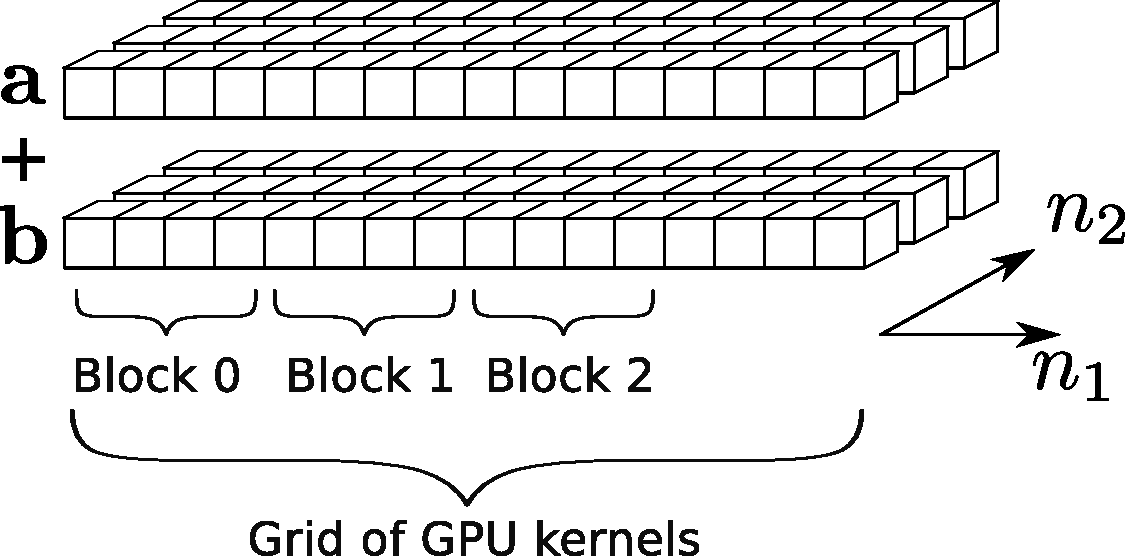
\includegraphics[scale=0.55]{Fig/abcgpu.pdf}
  \caption{Summation of vectors on GPU}
  \end{figure}
\end{frame}

\begin{frame}
  \ccode{35}{53}{gpuhello.c}{gpu/gpuhello.cu}
\end{frame}
\begin{frame}
  \ccode{54}{70}{gpuhello.c}{gpu/gpuhello.cu}
\end{frame}
\begin{frame}
  \ccode{71}{88}{gpuhello.c}{gpu/gpuhello.cu}
\end{frame}
\begin{frame}
  \ccode{87}{100}{gpuhello.c}{gpu/gpuhello.cu}
\end{frame}

\begin{frame}
  \begin{block}{How to compile}
    Look into RSFSRC/user/cuda/SConstruct 
  \end{block}
  \begin{block}{How to run}
    \$ scons/pscons
  \end{block}
  \begin{block}{Note}
    \begin{itemize}
      \item Can be launched on a multi-GPU cluster by {\bf pscons}
      \item Can be piped like a sequential Madagascar program
      \item You will need a dedicated GPU to run this code efficiently
      \item CUDA is proprietary
    \end{itemize}
  \end{block}
\end{frame}

\begin{frame}
  \begin{block}{Takeaway message}
    Exploit data parallelism when possible. It keeps programs simple and
    SConstructs portable.
  \end{block}
\end{frame}

